\subsection{Enhanced visualisation capabilities}

While writing \cite{viceeval}, Marcel already produced a simple off-line
support tool called \textit{``ShowVICE''}. This stand-alone tool is able
to display a UML sequence diagram (with time annotations) of the symbolic
execution of the VICE model.  This functionality is currently lacking
in VDMTools but it is essential for gaining insight into the model,
especially when concurrency and real-time issues come into play.
Such functionality should definitely become an integrated part of
VDMTools and should be enhanced further (for example adding a Gantt-chart
view of the active tasks in the model, showing instance variable evolution
over time etcetera). This kind of functionality provides important input
to the user for validating the correct behaviour of embedded systems.
It would also be valuable to have such sequence diagrams even in the
traditional VDM++ interpreter (without time information). Two screenshots
of the current ShowVice tool are provided in Figure~\ref{fig:sv1} and
Figure~\ref{fig:sv2}.

\begin{figure}[!htb]
\begin{centering}
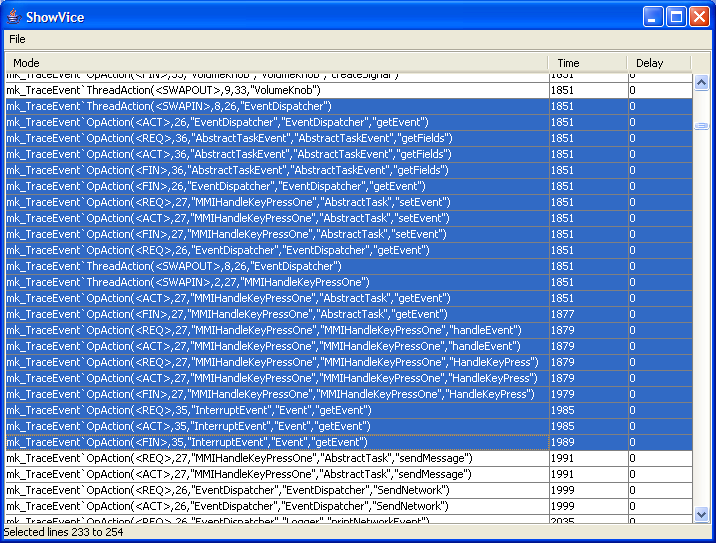
\includegraphics[width=0.80\textwidth]{showvice1.png}
\caption{The main user-interface of ``ShowVICE'', showing a parsed log file.}
\label{fig:sv1}
\end{centering}
\end{figure}

Figure~\ref{fig:sv1} shows an overview of the VICE trace file as it was
read back into the tool from the log file created by VICE after executing
the specification. The user can select the appropriate portion of the log
file that it wants to investigate, which is indicated by the highlighted
part of the list box.

\begin{figure}[!htb]
\begin{centering}
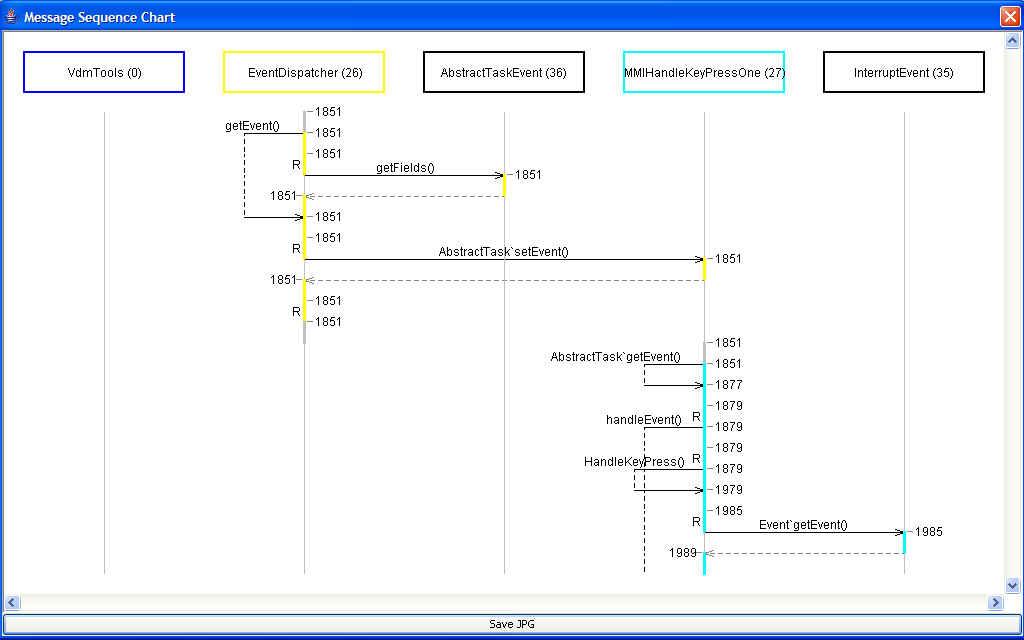
\includegraphics[width=\textwidth]{showvice2.png}
\caption{Detail screen showing a partial time annotated sequence diagram.}
\label{fig:sv2}
\end{centering}
\end{figure}

Figure~\ref{fig:sv2} shows the time annotated sequence diagram of the
selected portion of the trace file. In this particular diagram we see
that a context switch occurs between the \verb+EventDispatcher+ and
the \verb+MMIHandleKeyPressOne+ tasks. Also note that the execution of,
for example, the \verb+Event`getEvent+ operation takes exactly 4 time
units. This graphical feedback is essential to understand the behaviour
of the application. \\

When this kind of functionality is incorporated inside VDMTools, it would
also be extremely valuable to have support for predicates that can be
expressed over these traces. Typically these predicates will be expressed
with universal quantification and relating different events and the times
of their occurrences (inspired by predicates from Real Time Logic 
\cite{Jahanian&86}). It would
be valuable and save time for users if the tool is able to directly
demonstrate the counter-examples that did not satisfy the desired
predicate(s), preferably graphically as shown in Figure~\ref{fig:sv2}.
This is also the main reason why this visualisation functionality should
be integrated into VDMTools and not kept as an off-line inspection tool,
because when a predicate is invalidated, if possible the interpreter should
be stopped immediately such that the cause can be analysed by inspecting
the state of the model graphically as well as using the debugger
command-line. This possibility is obviously not available in the
off-line (post-simulation) based analysis.


